\section{Discussion}
\label{sec:discussion}

This section explores the underlying mechanisms of this collapse and its implications for Artificial General Intelligence (AGI). We deconstruct the failure into deficits across three core characteristics: (i) the violation of Modality-Agnosticism, evaluated via cross-modal performance comparisons; (ii) the breakdown of High-Level Cognition, analyzed through error attribution along the Understanding-Synthesizing-Reasoning (U/S/R) chain; and (iii) the absence of Open-ended Evolution, demonstrated by contrasting general LMs, fine-tuned LMs, and traditional architectures. Furthermore, (iv) we stress-test the models using few-shot learning to rule out shallow causes like insufficient context. Finally, we highlight the evolutionary bottlenecks in the current AGI trajectory and outline future directions.

\subsection{Cross-Modal Gap and the Violation of Modality-Agnosticism}

To evaluate the \textit{Modality-Agnostic} property, we analyze performance across the reasoning complexity gradient (MCQ, SCQ, TFQ). While elite models maintain a fragile reasoning facade in the textual modality, their cognitive capabilities catastrophically collapse in non-semantic environments. Astonishingly, massive LMs universally perform \textit{worse than random chance} across all metrics. The most glaring deficit occurs in the simplest binary task (TFQ, random baseline $56.74\%^\dagger$), where models like LLaVa-1.5 (Visual) and Vicuna-1.5 (Numerical) plunge to a mere $50.00\%$. As reasoning complexity increases, the capability gap widens to absurd proportions: on the visual MCQ, LLaVa-1.5 yields just $5.40\%$, and Llama-3.1 (70B) scores a dismal $6.40\%$ on the numerical MCQ. Both scores are less than half the $12.95\%^\dagger$ random baseline. This multi-dimensional, sub-random collapse definitively proves that current LMs lack genuine modality-agnosticism; their reasoning is heavily tethered to textual semantic shortcuts, completely failing to integrate raw physical signals.In stark contrast, specialized lightweight architectures provide compelling empirical proof for \textit{Representational Equivalence}. Despite processing radically different raw inputs, these models not only overwhelmingly crush their billion-parameter counterparts but also converge on nearly identical predictive distributions. Whether utilizing a Textual GRU, a Numerical CNN, or a Visual EfficientNet-B0, their accuracies universally stabilize across the entire gradient: peaking at $60\%$-$63\%$ on TFQ, $32\%$-$38\%$ on SCQ, and $19\%$-$25\%$ on MCQ. This flawless tri-modal convergence confirms that objective physical truths are invariant to sensory channels. It proves that once a model's architecture aligns with the physical world's structural logic, it can consistently extract identical macroscopic laws regardless of the data modality.


\subsection{U/S/R Capability Decomposition}


To gain deeper insight into the cognitive bottlenecks of High-Level Cognition (HLC), we decompose each incorrect prediction by identifying its most probable point of failure within the U/S/R pipeline. Following the formal attribution criteria detailed in Appendix~\ref{sec:usrules}, we quantify the proportion of errors assigned to the Understanding (U), Synthesizing (S), and Reasoning (R) stages for every model and modality. This diagnostic perspective serves as a vital complement to holistic accuracy: it reveals that models with comparable performance may nonetheless exhibit fundamentally distinct failure modes, exposing unique fractures along their internal cognitive chains. In the Textual modality, the majority of errors ($65.5\%$) are concentrated in the Reasoning (R) stage. This suggests that while LMs can maintain a facade of "understanding" by adhering to output constraints (low U-fail), they lack the underlying world model to execute correct physical deduction. However, as we shift to the Numerical and Visual modalities, we observe a surge in U-fail (reaching $46.7\%$ in Visual tasks). This indicates that raw physical signals act as "representational noise" that disrupts the models' instruction-following stability, causing them to abandon the requested output formats entirely. Furthermore, the high S-fail in the Numerical modality ($31.8\%$) reflects a profound internal logical dissonance, where models simultaneously generate mutually exclusive physical states. These findings empirically confirm that LMs' failures are not merely "wrong answers" but a fundamental breakdown of the entire cognitive pipeline when stripped of semantic scaffolding.


% We further attribute each incorrect prediction to the most likely broken cognitive stage under MHLC. The U/S/R rules used for this attribution are defined in Appendix~\ref{sec:usrules}. Conceptually:
% \begin{itemize}
%     \item \textbf{Understanding (U)} focuses on interpreting fragmented non-semantic evidence.
%     \item \textbf{Synthesising (S)} focuses on integrating evidence into an implicit global framework.
%     \item \textbf{Reasoning (R)} focuses on mapping the global framework to high-level tactical style labels.
% \end{itemize}

% Practically, we compute the fraction of errors attributed to U/S/R for each model and modality. This produces an error-composition view complementary to end-task accuracy: two models with similar accuracy can differ substantially in *where* they fail along the chain.



\subsection{The Stagnation of Open-Ended Evolution}
In the context of solving specific physical-world problems, the model training process essentially serves as a mechanism to approximate the performance upper bound for a given task. Empirical results demonstrate that traditional architecture models establish a clear performance baseline through training, representing the physical upper bound of the "passive fitting" capacity on specific data distributions within traditional AI paradigms. However, a compelling phenomenon emerges: despite undergoing equivalent training regimes, Large Models (LMs) not only fail to surpass but comprehensively underperform compared to traditional architecture models. This performance inversion exposes profound architectural limitations within LMs: they are fundamentally incapable of efficiently achieving passive fitting to specific physical dynamics, even within closed environments. Following an a fortiori argument, Open-ended Evolution necessitates that an intelligent agent continuously and precisely assimilates and restructures novel knowledge through active interaction within complex physical environments. If LMs are architecturally precluded from even reaching the static upper bound of passive fitting, this constitutes powerful counter-evidence: they currently lack the fundamental capacity to achieve continuous, open-ended evolution through real-world physical interactions.








% Section~\ref{sec:experiment} established the main quantitative picture: large LMs and VLMs remain at random-level on MHLC even after MatchIntel2 fine-tuning, while tiny specialized architectures solve the task far better---evidence that scale alone does not realize multimodal high-level cognition toward physical-world evidence. Section~\ref{sec:experiment} also summarized collapse severity across modalities and scales at a statistical level. This section turns to \emph{why} that collapse arises and what it implies for Artificial General Intelligence (AGI): we (i) articulate the MHLC failure as a breakdown of the full U$\rightarrow$S$\rightarrow$R chain rather than a dataset artifact, (ii) decompose errors along U/S/R to mirror our definition of generalizable physical-world cognition, (iii) stress-test two common ``fixes''---more demonstrations and more parameters---to exclude superficial explanations, and (iv) outline future directions that target domain and architectural depth rather than incremental fitting.

% \subsection{MHLC Collapse and the Limits of Dataset Fitting}
% Under MHLC, inputs are non-semantic numerical sequences and spatial heatmaps, while targets remain high-level tactical style labels. The key scientific question is whether the HLC gains seen in textual modality are \emph{intrinsic} and modality-agnostic, or whether they mainly arise from semantic shortcut learning that cannot survive when linguistic scaffolding is removed.

% The main results already support the second reading at the level of end-task accuracy: the same PEFT recipe that lifts textual HLC leaves numerical and visual MHLC at chance. That pattern is difficult to reconcile with ``the model only needed more in-domain examples'': MatchIntel2 supervision is available, yet general LMs do not acquire stable U$\rightarrow$S$\rightarrow$R over raw non-semantic observations. We therefore interpret collapse as reflecting a \emph{structural} deficit---how these models represent and integrate physical evidence---rather than a temporary optimization gap solvable by better loss landscapes on the same architecture.

% To move from this qualitative claim to a finer-grained view, we decompose incorrect behaviour into failure modes aligned with the U/S/R cognitive chain. The statistics in Table~\ref{tab:failure_modes_placeholder} are computed from saved raw outputs and evaluation traces (TBD in your post-processing).

% Interpretation guidance (to be instantiated by your final numbers):
% \begin{itemize}
%     \item If general LLM/VLM failures are dominated by U- or S-stage attribution, it supports the view that non-semantic inputs prevent the formation of the implicit global framework required by MHLC.
%     \item If R-stage failures remain high even when U/S appear partially preserved, it suggests that mapping the synthesized global framework into tactical style labels requires architectural or inductive bias not provided by parameter-only fine-tuning.
%     \item If lightweight models show a different U/S/R breakdown (e.g., fewer failures in earlier stages), it directly supports the claim that specialized architectures better instantiate the MHLC chain over non-semantic evidence.
% \end{itemize}

\begin{table}[t]
    \centering
    \caption{Placeholder: Failure-mode breakdown from raw output logs. Each cell is TBD and will be filled with your computed statistics.}
    \label{tab:failure_modes_placeholder}
    \renewcommand{\arraystretch}{1.15}
    \setlength{\tabcolsep}{6pt}
    \begin{tabular}{l c c c c}
        \toprule
        \textbf{Model} & \textbf{Mod.} & \textbf{U-fail} & \textbf{S-fail} & \textbf{R-fail} \\
        \midrule
        General LMs (Zero-shot) & Tex. & 12.4\% & 22.1\% & 65.5\% \\
        General LMs (Zero-shot) & Num. & 28.7\% & 31.8\% & 39.5\% \\
        General LMs (Zero-shot) & Vis. & 46.7\% & 16.3\% & 37.0\% \\
        \bottomrule
    \end{tabular}
\end{table}



% \begin{figure}[t]
%     \centering
%     \fbox{
%         \parbox{0.95\linewidth}{
%         \textbf{Placeholder Figure: U/S/R attribution distribution.}\\
%         Suggested content: stacked bars for (Num vs Vis) and (Zero-shot vs PEFT vs Lightweight), with segments U/S/R.\\
%         Data: TBD (to be filled using your log-based statistics).\\
%         Caption idea: ``U/S/R-wise failure composition across models and modalities under MHLC.''
%         }
%     }
%     \caption{Placeholder for U/S/R-wise error composition.}
%     \label{fig:usr_attribution_placeholder}
% \end{figure}

% \subsection{Ruling Out Shallow Explanations: Prompting and Parameter Scale}
% Beyond fine-tuning, two frequent suspicions are that collapse is due to insufficient task context or to insufficient model capacity. We briefly stress-test both; full plots are kept for transparency, but the takeaway is that neither removes the MHLC bottleneck.

% \subsubsection{Can Few-Shot Prompting Activate Cognition?}
% A hypothesis is that a model might fail in a zero-shot setting simply due to insufficient task context, and that providing demonstration examples via Few-Shot Learning (FSL) could activate MHLC. To investigate this, we prompt LMs with 0-shot, 1-shot, and 2-shot demonstrations in both visual and numerical modalities. As shown in Figure \ref{fig:few_shot_ablation}, increasing demonstrations only causes marginal and random fluctuations, rather than consistent improvement. For example, in the numerical modality, Llama-3.3-70B-Instruct achieves 0.074 and 0.068 on MCQ under 1-shot and 2-shot, respectively, still below the 0.118 threshold. A similar trend appears in the visual modality, where Gemma-3-27B-IT reaches only 0.068 on MCQ under 2-shot.

% By inspecting generated responses, we observe that demonstrations can improve template compliance (i.e., fewer invalid/unformatted outputs), but candidate selection remains random. This indicates that FSL provides surface-level alignment without enabling the required cognitive integration. Therefore, the MHLC bottleneck is not lack of prompt context, but intrinsic cognitive deficit under non-semantic conditions.

% \begin{figure}[t!]
% 	\centering
% 	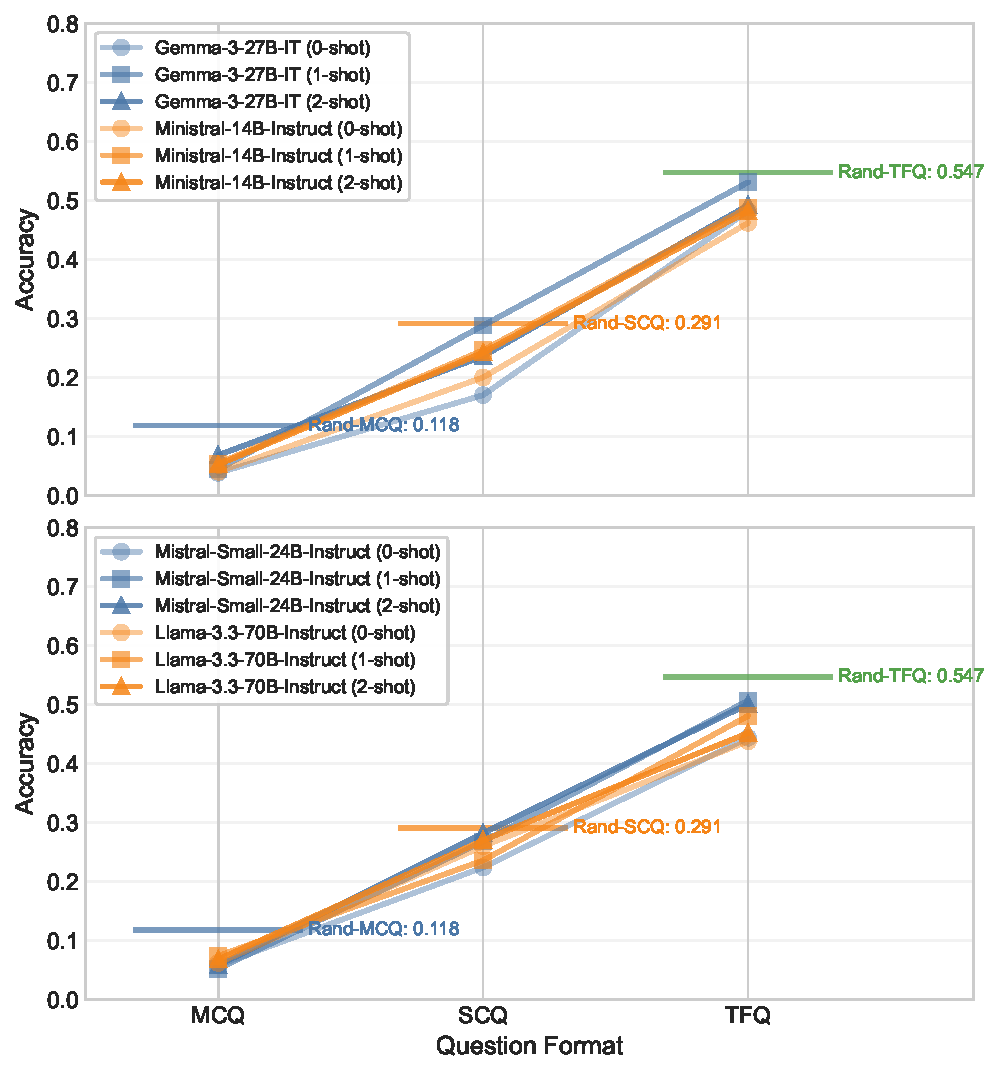
\includegraphics[width=\linewidth]{figure/ablation_fewshot_v2.pdf}
% 	\caption{Few-shot ablation in visual and numerical modalities (data from Experiment2). Colored reference lines indicate random-level thresholds for MCQ, SCQ, and TFQ. Performance fluctuations remain near random-level, showing no stable cognitive gain from additional demonstrations.}
% 	\label{fig:few_shot_ablation}
% \end{figure}

% \subsubsection{Can Scaling Up Bridge the Cognitive Gap?}
% Another assumption is that poor performance after fine-tuning may be caused by insufficient parameter scale, and that larger models might capture non-semantic features better. To test this, we evaluate fine-tuned models across parameter scales (1B--13B) and model families (Llama, Qwen, and LLaVA) in both visual and numerical modalities. As shown in Figure \ref{fig:scaling_ablation}, scaling up does not yield consistent gains.

% In the visual modality, increasing LLaVA-1.5 from 7B to 13B slightly decreases MCQ/SCQ/TFQ performance (0.116/0.194/0.514 vs. 0.114/0.172/0.482). In the numerical modality, scaling Llama-3.2 from 1B to 3B keeps TFQ unchanged at 0.492, while Qwen-2.5-7B remains near random-level with TFQ at 0.538. These results indicate that larger parameter scales do not inject intrinsic MHLC and cannot bridge the cognitive gap in non-semantic modalities.

% \begin{figure}[t!]
% 	\centering
% 	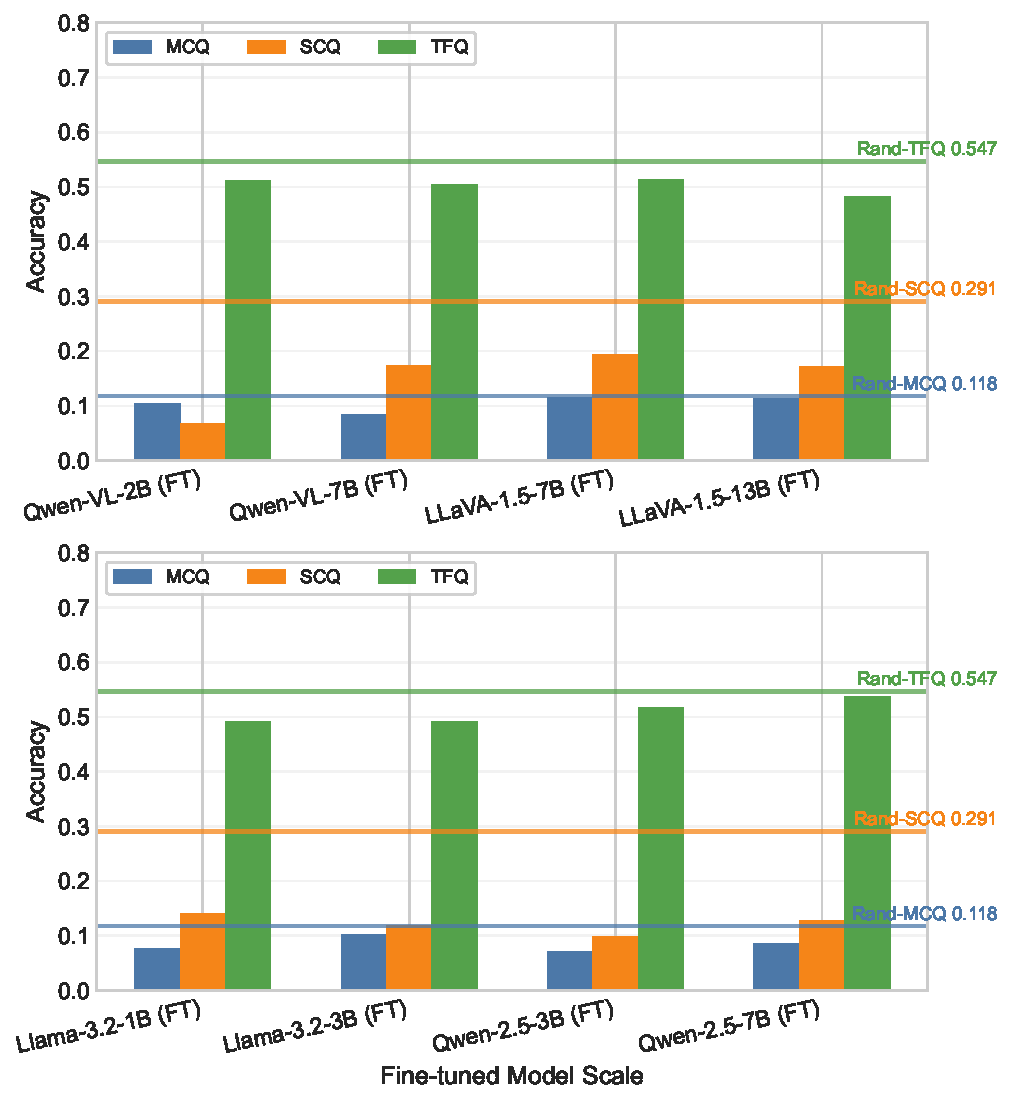
\includegraphics[width=\linewidth]{figure/ablation_scaling_v2.pdf}
% 	\caption{Scaling ablation in visual and numerical modalities (data from Experiment3). Colored reference lines indicate random-level thresholds. Increasing parameter scale under fine-tuning does not produce stable improvements toward MHLC.}
% 	\label{fig:scaling_ablation}
% \end{figure}

% \subsection{Future Directions}
% The evidence above pushes AGI-relevant multimodal cognition out of the ``scale and prompt engineering'' comfort zone. If the goal is systems that perceive and reason about the physical world across modalities, then MHLC-style tasks surface three concrete research fronts. First, \textbf{non-semantic grounding}: architectures need inductive biases (temporal-spatial structure, long-horizon aggregation, uncertainty over latent match state) that current conversational LMs do not obtain from text-heavy pre-training alone. Second, \textbf{evaluation beyond accuracy}: U/S/R attribution should evolve from heuristic rules to calibrated probes and controlled interventions (e.g., counterfactual trajectories, partial observability ablations) so that failure is diagnosable, not only binary. Third, \textbf{domain depth}: soccer is one instantiation; transferring the same U$\rightarrow$S$\rightarrow$R contract to other physical domains (robotics logs, environmental sensing, clinical time series) tests whether insights are general or sport-specific. Closing the gap between lightweight specialists and general LMs likely requires co-design of data interfaces, objectives, and architectures---not incremental fitting on the same templates.

% Practical limitations of the present study (compute scope, model families, and modality coverage) are summarized alongside a shorter forward-looking note in Appendix~\ref{sec:limitations}.
